\documentclass[12pt,a4paper]{article}
\usepackage{amsmath,amscd,amsbsy,amssymb,latexsym,url,bm,amsthm}
\usepackage{epsfig,graphicx,subfigure}
\usepackage{enumitem,balance}
\usepackage{wrapfig}
\usepackage{mathrsfs,euscript}
\usepackage[usenames]{xcolor}
\usepackage{hyperref}
\usepackage[vlined,ruled,linesnumbered]{algorithm2e}
\hypersetup{colorlinks=true,linkcolor=black}

\newtheorem{theorem}{Theorem}
\newtheorem{lemma}[theorem]{Lemma}
\newtheorem{proposition}[theorem]{Proposition}
\newtheorem{corollary}[theorem]{Corollary}
\newtheorem{exercise}{Exercise}
\newtheorem*{solution}{Solution}
\newtheorem{definition}{Definition}
\theoremstyle{definition}

\renewcommand{\thefootnote}{\fnsymbol{footnote}}

\newcommand{\postscript}[2]
 {\setlength{\epsfxsize}{#2\hsize}
  \centerline{\epsfbox{#1}}}

\renewcommand{\baselinestretch}{1.0}

\setlength{\oddsidemargin}{-0.365in}
\setlength{\evensidemargin}{-0.365in}
\setlength{\topmargin}{-0.3in}
\setlength{\headheight}{0in}
\setlength{\headsep}{0in}
\setlength{\textheight}{10.1in}
\setlength{\textwidth}{7in}
\makeatletter \renewenvironment{proof}[1][Proof] {\par\pushQED{\qed}\normalfont\topsep6\p@\@plus6\p@\relax\trivlist\item[\hskip\labelsep\bfseries#1\@addpunct{.}]\ignorespaces}{\popQED\endtrivlist\@endpefalse} \makeatother
\makeatletter
\renewenvironment{solution}[1][Solution] {\par\pushQED{\qed}\normalfont\topsep6\p@\@plus6\p@\relax\trivlist\item[\hskip\labelsep\bfseries#1\@addpunct{.}]\ignorespaces}{\popQED\endtrivlist\@endpefalse} \makeatother

\begin{document}
\noindent

%========================================================================
\noindent\framebox[\linewidth]{\shortstack[c]{
\Large{\textbf{Lab06-Graph Exploration}}\vspace{1mm}\\
CS214-Algorithm and Complexity, Xiaofeng Gao, Spring 2019.}}


\begin{center}
\footnotesize{\color{red}$*$ If there is any problem, please contact TA Mingran Peng.}\par
% Please write down your name, student id and email.
\footnotesize{\color{blue}$*$ Name:KylinChen \quad Student ID:517030910155 \quad Email: k1017856853@icloud.com}
\end{center}
\begin{enumerate}
    
    \item
    Given a graph, find the number of Strongly Connected Components in the graph.
    \begin{enumerate}
        \item
         Complete the implementation in the provided C/C++ source code. Notice that in the source code there will be more detailed explanation.{\color{blue}(The source code \emph{SCC.cpp} is attached on the course webpage.)}\par
       \item
        Use the $Gephi$ to draw the graph. If you think the data provided is not beautiful, you can generate your own data. Notice that result of $Gephi$ will be taken into consideration of Best Lab.\par 
        
    \end{enumerate}
    \begin{solution}\item
        \renewcommand{\qedsymbol}{}
        \begin{itemize}
        \item \textbf{(a)} Code file \emph{SCC.cpp} is attached in the .zip file.
        \item \textbf{(b)} In this problem, we use python to extract data from \emph{scc.in} to generate data.xlsx. Then we can import the .xlsx into $Gephi$ to draw the graph. Data-Operation file(main.py), Model file(prob1.gephi), Data file(data.xlsx) is attached in $/materials$ content.\par
        One of generated graph can be as Graph.~\ref{Graph0}.

        \begin{figure}[htbp]
        \centering
        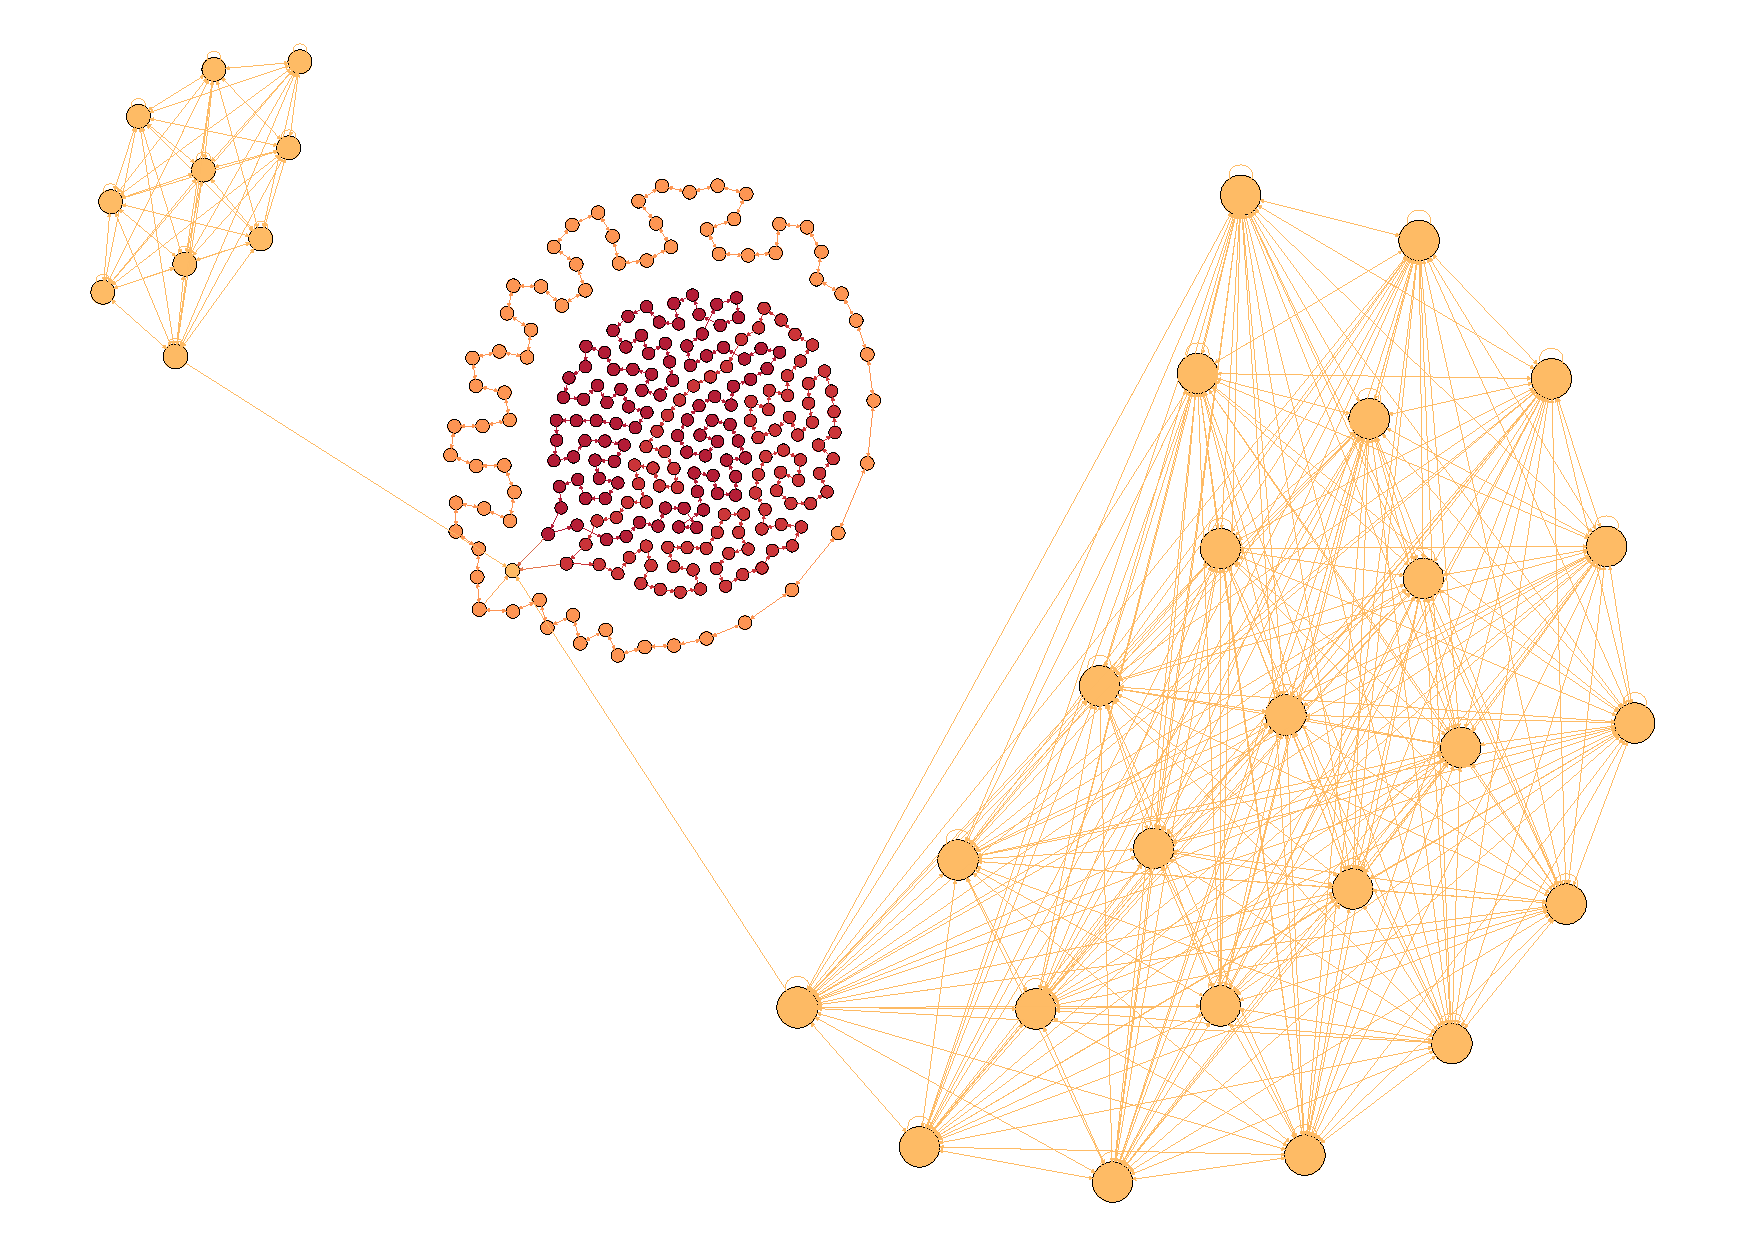
\includegraphics[width=0.8\textwidth]{pictures/pic_0.pdf}
        \caption{\textbf{Generated Graph by Gephi}}\label{Graph0}
        \end{figure}
        \end{itemize}
    \end{solution}


\item
    Remember the lemma introduced in the course: : $\forall u, v \in V$, intervals $[PRE(u), POST(u)]$, $[PRE(v), POST(v)]$ are either disjoint or one is contained within the other.\par
Prove the lemma.\par
    \begin{proof}
        \renewcommand{\qedsymbol}{}
        This lemma and its proof relies on the Algorithm.~\ref{ALG1} and Algorithm.~\ref{ALG2} below:\item
        \begin{minipage}[t]{0.9\textwidth}
        \begin{algorithm}[H]
            \KwIn{$G = (V, E)$ is a graph; $v \in V$}
            \KwOut{$VISITED(u) = true$ for all nodes $u$ reachable from $v$}
            %\BlankLine
            \caption{$EXPLORE(G, v)$}
            \label{ALG1}
            \BlankLine
            $VISITED(v) = true$\;
            $PREVISIT(v)$\;
            \For{each $edge(v,u)\in E$}{
                \If{not $VISITED(u)$}{
                    $EXPLORE(G, u)$\;
                }

            }
            $POSTVISIT(v)$\;
        \end{algorithm}
        \end{minipage}
        \hfill


        \begin{minipage}[t]{0.9\textwidth}
        \begin{algorithm}[H]
            \KwIn{$G = (V, E)$ is a graph}
            \KwOut{$VISITED(v)$ is set to true for all nodes $v \in V$}
            %\BlankLine
            \caption{$DFS(G)$}
            \label{ALG2}
            \BlankLine
            
            \For{each $v \in V$}{
                $VISITED(v) = false$\;
            }

            \For{each $v \in V$}{
                \If{not $VISITED(v)$}{
                    $EXPLORE(G, v)$\;
                }
            }
        \end{algorithm}
        \end{minipage}
        \hfill
        \item
        We can easily simplify the relationship between point $v$ and $u$ as three model in Graph.~\ref{Graph1}
        
        \textbf{Model Explanation:} 
        \begin{itemize}
        \item According to symmetry, we can define DFS Algorithm access ordering is: $p \rightarrow u \rightarrow v$ or $u \rightarrow v$ (if p doesn't exist).
        \item Dash line means there exist only one disjoint path (don't have same points in another path or available paths are accessed before) between these two points. 
        \item Full line means there exist path between these two points (a stronger constrain than last one).
        \item No line means there doesn't exist any path or all available paths are accessed before between these two points.
        \item $p$ is some arbitrary point besides $u$ and $v$, if there exist $p'$ have full line from $p$ to $u$, it means these model(2) is model(1) actually.
        \item We can easily find that all the relationship between point $u$ and $v$ can be simplified into these three formats and they are matually exclusive.
        \end{itemize}
        \begin{figure}[htbp]
        \centering
        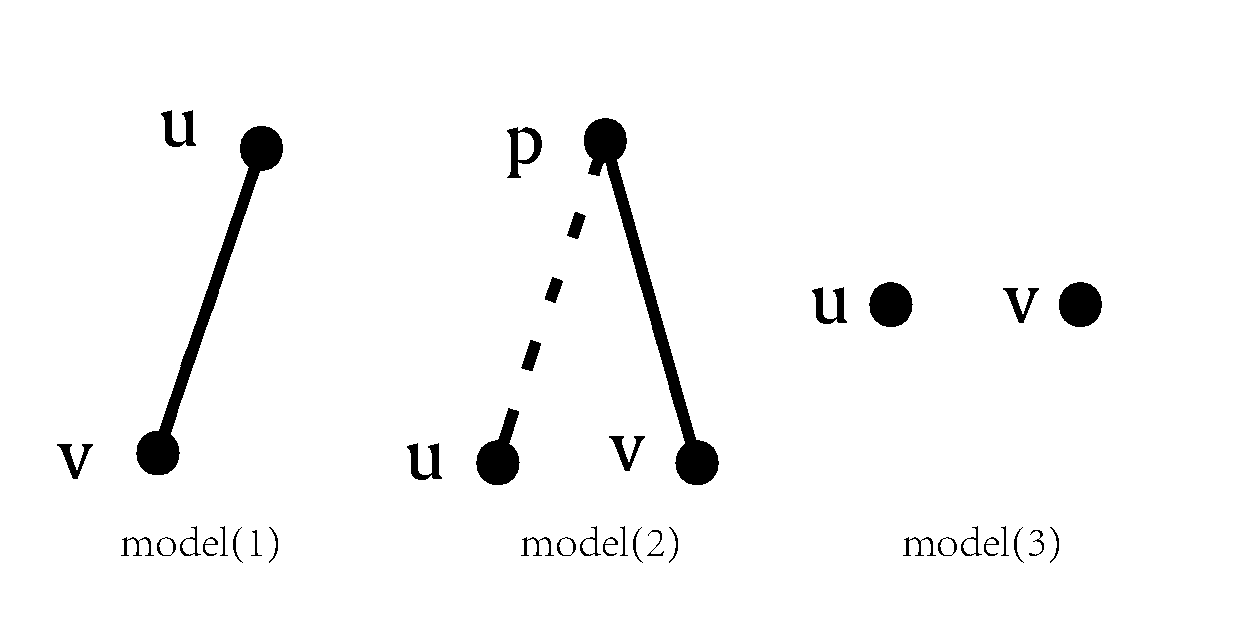
\includegraphics[width=0.6\textwidth]{pictures/pic_1.pdf}
        \caption{\textbf{Simplified Models}}\label{Graph1}
        \end{figure}\item

        Now, we will give interval relationship between $[PRE(u), POST(u)]$ and $[PRE(v), POST(v)]$ for every model:\item
        \begin{itemize}
          \item In \textbf{model(1)}, refering to Algorithm.~\ref{ALG1}, once we call EXPLORE$(G,u)$ it will recurrsively call EXPLORE$(G, v)$, and EXPLORE$(G, u)$ start before EXPLORE$(G, v)$, EXPLORE$(G, v)$ terminate before EXPLORE$(G, u)$, it means [$PRE(v)$, $POST(v)$] is contained by [$PRE(u)$, $POST(u)$].
          \item In \textbf{model(2)}, once we call EXPLORE$(G, u)$, it can't recurrsively call EXPLORE$(G, v)$ because there are no available path for it. In this case, refering to Algorithm.~\ref{ALG2}, we will call
           DFS$(G)$ to find another explore beginning point. Therefore, EXPLORE$(G, u)$ terminate before we call EXPLORE$(G, v)$, it means [$PRE(v)$, $POST(v)$] is disjoint with [$PRE(u)$, $POST(u)$].
          \item In \textbf{model(3)}, similarly, once we call EXPLORE$(G, u)$, it can't recurrsively call EXPLORE$(G, v)$ because there are no available path for it. In this case, refering to Algorithm.~\ref{ALG2}, we will call
           DFS$(G)$ to find another explore beginning point in another connected component. Therefore, EXPLORE$(G, u)$ terminate before we call EXPLORE$(G, v)$, it means [$PRE(v)$, $POST(v)$] is disjoint with [$PRE(u)$, $POST(u)$].
        \end{itemize}
        As is mentioned above, $\forall u, v \in V$, intervals $[PRE(u), POST(u)]$, $[PRE(v), POST(v)]$ are either disjoint or one is contained within the other.\par

    \end{proof}
\item
Consider there is a network consists $n$ computers. For some pairs of computers, a wire exists in the pair, which means these two computers can communicate with delay $t$.\par
Assume that computer $s$ wants to issue a message to computer $t$, we want to know the minimum time needed to send this message.\par
You need to provide the pseudo code and analyze the time complexity.\par

    \begin{solution}
        \renewcommand{\qedsymbol}{}
        We can use Improved-BFS-Algorithm or Dijkstra-Algorithm to solve this problem, their pseudo code and analyze are follows:\par

        \textbf{(1) Improved-BFS-Algorithm:}\item
        \begin{minipage}[t]{0.9\textwidth}
        \begin{algorithm}[H]
            \KwIn{$G = (V, E)$ is a graph; $s, t \in V$;}
            \KwOut{Minimal weighted route from $s$ to $t$;}
            %\BlankLine
            \caption{Improved-BFS-Algorithm}
            \label{ALG3}
            \BlankLine
            $Res[|V|]$\;
            \For{each $i \in |V|$}{
                $Res[i]=\infty$\;
            }
            $Res[t]\leftarrow 0$\;
            $Queue\rightarrow [\ ]$\;
            $enqueue(Queue,s)$\;
            \While{Not $empty(Queue)$}{
                $v = dequeue(Queue)$\;
                \For{each $p$ connect $v$}{
                    \If{$Res[v]+t<Res[p]$}{
                        $Res[p]=Res[v]+t$\;
                        $enqueue(Queue,p)$\;
                    }
                }
            }
            \Return{Res[t]}\;
        \end{algorithm}
        \end{minipage}
        \hfill
        \item\item\item
        \textbf{(2) Dijkstra-Algorithm:}\item
        \begin{minipage}[t]{0.9\textwidth}
        \begin{algorithm}[H]
            \KwIn{$G = (V, E)$ is a graph; $s, t \in V$;}
            \KwOut{Minimal weighted route from $s$ to $t$;}
            %\BlankLine
            \caption{Dijkstra-Algorithm}
            \label{ALG4}
            \BlankLine
            $C \leftarrow \{s\}$\;
            $Res[|V|]$\;
            \For{each $i \in |V|$}{
                $Res[i]=\infty$\;
            }
            $Res[t]\leftarrow 0$\;
            \While{$V$ and $V-C$ are connected}{
                $Tmp\leftarrow \{\}$\;
                \For{each $p \in |V-C|$ which links $w$ in $C$}{
                    $Tmp\leftarrow Tmp\cup\{p\}$\;
                    $Res[p]=Min{Res[p],Res[w]+ t}$\;
                    $k=Min(Res[\forall\ i\ in\ Tmp])$\;
                    $C\leftarrow C\cup\{k\}$\;
                }
            }
            \Return{Res[t]}\;
        \end{algorithm}
        \end{minipage}
        \hfill
        
        \textbf{Complexity Analysis:}\item
        We first define the unity time cost as we access an edge or a point.
        \begin{itemize}
        \item \textbf{Improved-BFS-Algorithm:} Now that BFS access all the points in the graph and access all the edges(include check unavailable edges), we can find the Time Complexity is $O(|V| + |E|)$.
        \item \textbf{Dijkstra-Algorithm:} Time Complexity relies on the data structure we use. As for row 6 and row 11 in Algorithm.~\ref{ALG4}. How we find the minimal-distance point determine the time complexity.\par
        \textbf{(1)} If we use matrix to store the vertex relationship and use brute travel method, for each vertex we will check all the $|V|-1$ vertices, it means the Time Complexity is $O(|V|^2)$.
        \par
        \textbf{(2)} If we use a binary heap to find the minimal-distance vertex for each point in graph, we can transmute the algorithm into BFS and binary heap insertion in each step, which means the Time Complexity is $O((E+N)logN)$.
        \par
        \textbf{(3)} If we use fibonacci heap to find the minimal-distance vertex for each point in graph, we can get a optimized Time Complexity  $O(NlogN+E)$.
        \par
        \end{itemize}

    \end{solution}


    

\end{enumerate}

\vspace{20pt}

%========================================================================
\end{document}
